\documentclass[12pt,a4paper]{article}
\usepackage[spanish]{babel}
\usepackage[utf8]{inputenc}

\usepackage[right=2cm,left=3cm,top=2cm,bottom=2cm,headsep=0cm,footskip=0.5cm]{geometry}
\usepackage{graphicx,subfigure}
\usepackage{amsmath}
\usepackage{underscore}

\graphicspath{ {img/} }

\title{\textbf{Uso de redes sociales: ventajas e inconvenientes}}
\author{Alberto Navalón Lillo}

\begin{document}

\maketitle
\tableofcontents

\section{Introducción}

Las \textbf{redes sociales} se han convertido en los últimos tiempos en una herramienta esencial para nuestra vida social actual. Con la creación de Internet a finales del siglo XX, conectar a personas de lugares distintos e incluso muy remotos se ha ido convirtiendo en una tarea cada vez más sencilla. Aprovechando estas nuevas ventajas, desarrolladores crearon plataformas en línea donde se podían comunicar individuos a mucha distancia, y en algunas ocasiones de manera casi instantánea. Un ejemplo de estas plataformas primitivas, y que aún están muy extendidas, fueron los foros virtuales.\\

A partir de estas primeras plataformas, la funcionalidad de las mismas se fue aumentando, al igual que su capacidad y su extensión en la sociedad. A raíz de estas mejoras surgió el concepto de \textit{redes sociales}. Actualmente, podemos encontrar redes sociales de muchas clases, desde \textbf{mensajería instantánea} (WhatsApp, Telegram, Facebook Messenger...) hasta \textbf{chats de vídeo} (Skype, Discord...), pasando por otras muy conocidas, como YouTube, Facebook, Twitter, Instagram, o todo tipo de blogs. Fácilmente podemos observar cómo las redes sociales han aumentado considerablemente su complejidad, que puede llegar a ser abrumadora a la hora de hacer uso de ellas. La creación de nuevos productos alrededor de estas plataformas nos hace mantenernos más tiempo pegados a las pantallas, siendo las empresas propietarias las únicas beneficiarias de su consumo abusivo por parte de la población, que no puede dar abasto a la hora de hacer uso de estos nuevos productos, que aparentemente son beneficiosos, pero realmente provocan más mal que bien.\\

Es gracias a esta creciente variedad y diversificación de las redes lo que ha provocado que en los últimos años, el porcentaje de población registrada en estas plataformas y sitios web haya aumentado drásticamente, hasta el punto en que estas redes han alcanzado una penetración del 85\%\footnote{``Estudio anual de redes sociales 2019'', IAB Spain.\\https://iabspain.es/estudio/estudio-anual-de-redes-sociales-2019/} en España, como se puede observar en el siguiente gráfico de barras (\textit{Fig. A}):\\

\begin{figure}[h]
	\centering
	\subfigure[Fig. A: Evolución de la penetración del uso de redes sociales en España entre los años 2009 y 2019. \textit{Fuente: IAB Spain}.]{\label{fig:a}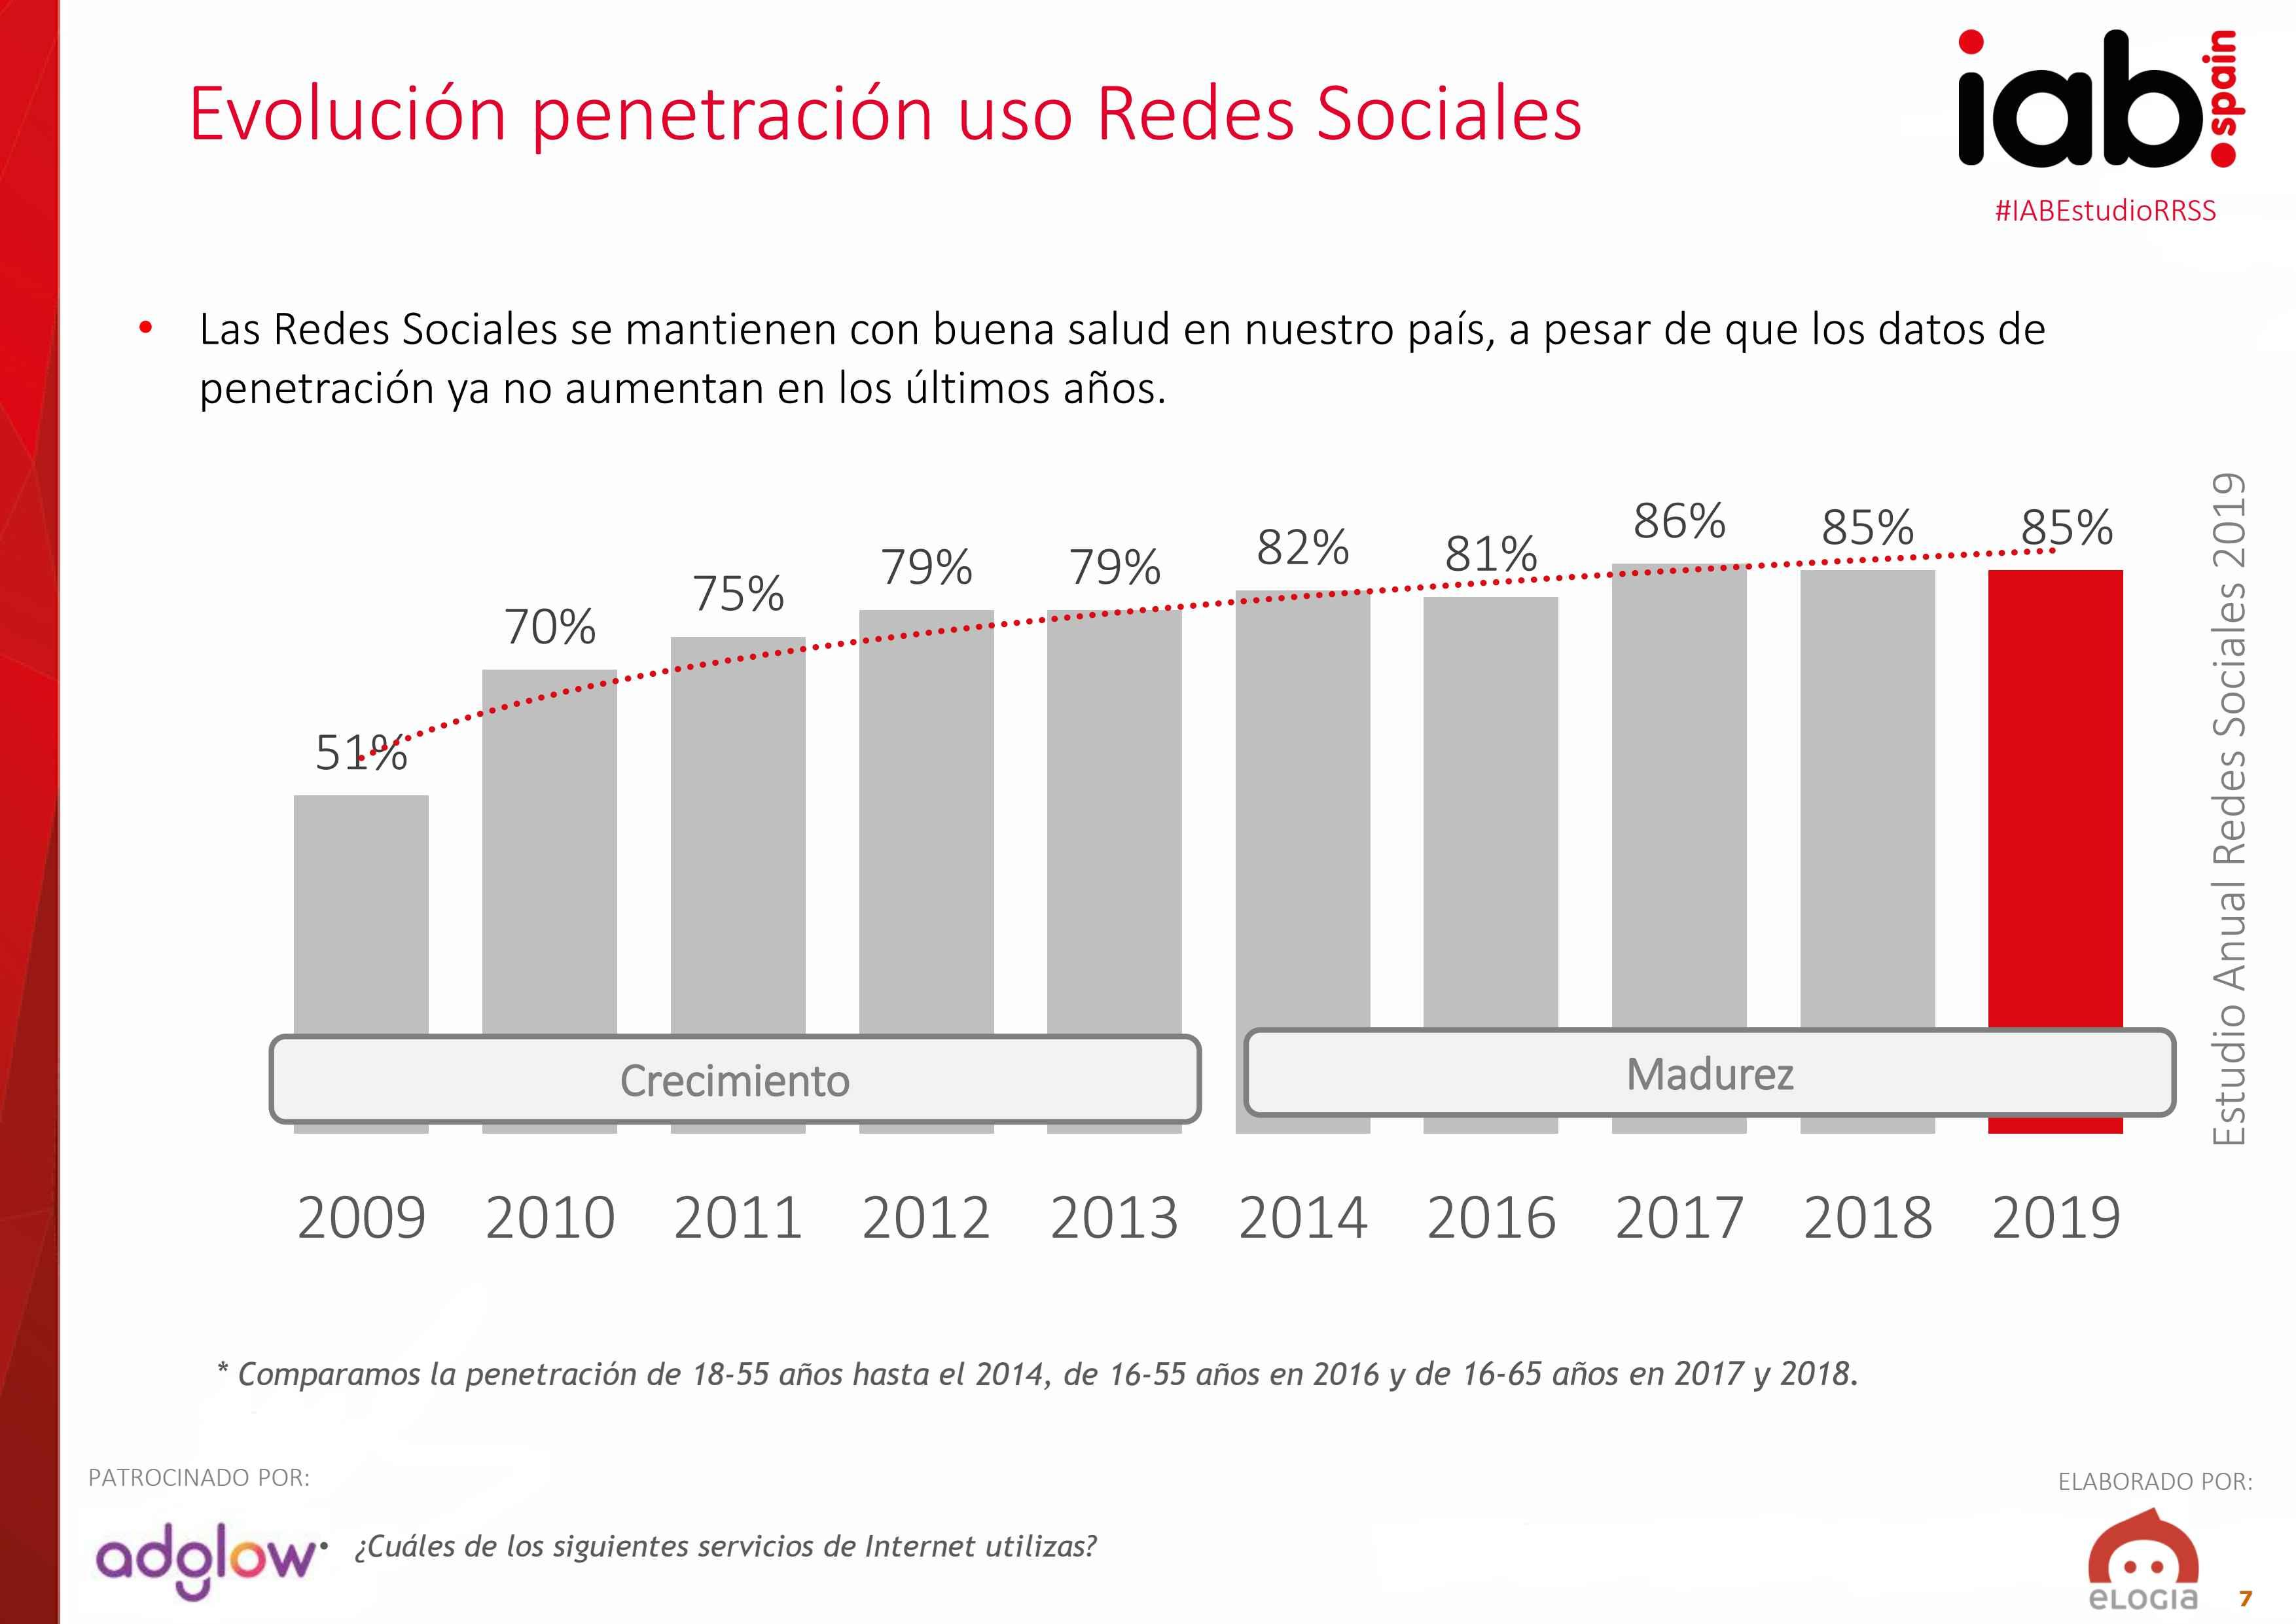
\includegraphics[width=120mm]{penetracion-rrss-espana}}
\end{figure}

A continuación, procederemos a explicar las diferentes ventajas e inconvenientes del uso de las redes sociales, dejando un apartado exclusivo para cada uno de estos grupos.

\section{Redes sociales}

\subsection{Ventajas}

Dentro de las múltiples ventajas que estas nuevas tecnologías ofrecen, posiblemente la más significativa sea la posibilidad de contactar con gente, tanto si son familiares, amigos, conocidos o incluso desconocidos, sobre todo si viven lejos de ti, de forma que se convierten en una herramienta muy útil. Además, todo este contacto se produce de forma inmediata, al igual que se puede recibir una ingente cantidad de información de cualquier aspecto instantáneamente.\\

Otras ventajas que este mundo virtual ofrece son el poder compartir experiencias con el mundo, como por ejemplo, tuiteando, subiendo un vídeo a YouTube, o escribiendo en un blog; romper las barreras culturales, dado que en internet podemos encontrar contenido de prácticamente cualquier lugar del mundo, de forma que podemos aprender del modo de vida de la gente al otro lado del planeta, al igual que de su cultura, costumbres, o incluso religión; encontrar pareja, en plataformas como Tinder o Meetic, y por último, siendo esta una de las mejores ventajas en mi opinión: la formación. Podemos encontrar todo tipo de recursos de aprendizaje en internet, tanto gratuitos como de pago, hasta el punto en el que te puedes formar de la misma forma o incluso mejor que realizando una carrera universitaria.

\subsection{Desventajas}

Al igual que las redes sociales comportan un gran número de ventajas, también pueden conllevar diversas desventajas o incluso peligros si no se hace un uso responsable de ellas. Por ejemplo, en estas plataformas podemos ser víctimas de delitos como el \textit{ciberbullying} o \textbf{ciberacoso}, sobre todo si se trata de menores, en los que ser víctima de este delito puede llegar a ser objeto de trastornos psicológicos. Otro delito frecuente que se produce en las redes es la \textbf{suplantación de identidad}, también denominada \textit{grooming}, que comúnmente se practica para chantajear a los usuarios para obtener material comprometedor.\\

Fuera de los ciberdelitos, el usar estas tecnologías irresponsablemente nos puede afectar personalmente de distintas formas, entre ellas, provocándonos una adicción a su uso, que suele ser muy prolongado, incluso si no se es adicto, con lo cual se reduce considerablemente nuestra productividad.\\

Para finalizar, me gustaría mencionar dos conceptos: la \textit{desconexión social} y la \textit{desinformación}. Este primero es muy frecuente, y trata de desvincular emocionalmente a las personas de sus contactos, dado que la comunicación y sus relaciones se reducen únicamente a las redes, sin ninguna relación física. En segundo lugar, la desinformación va cada vez más en aumento, a medida que surgen más y más bulos, hasta el punto que se nos hace casi imposible distinguir entre la información veraz y la falsa, ya que toda ella llega a un nivel de verosimilitud realmente excepcional.

\subsection{Uso de redes sociales en España}

\begin{figure}[h]
	\centering
	\subfigure[Fig. B: Uso de las principales redes sociales en España. Año 2019. \textit{Fuente: IAB Spain}.]{\label{fig:b}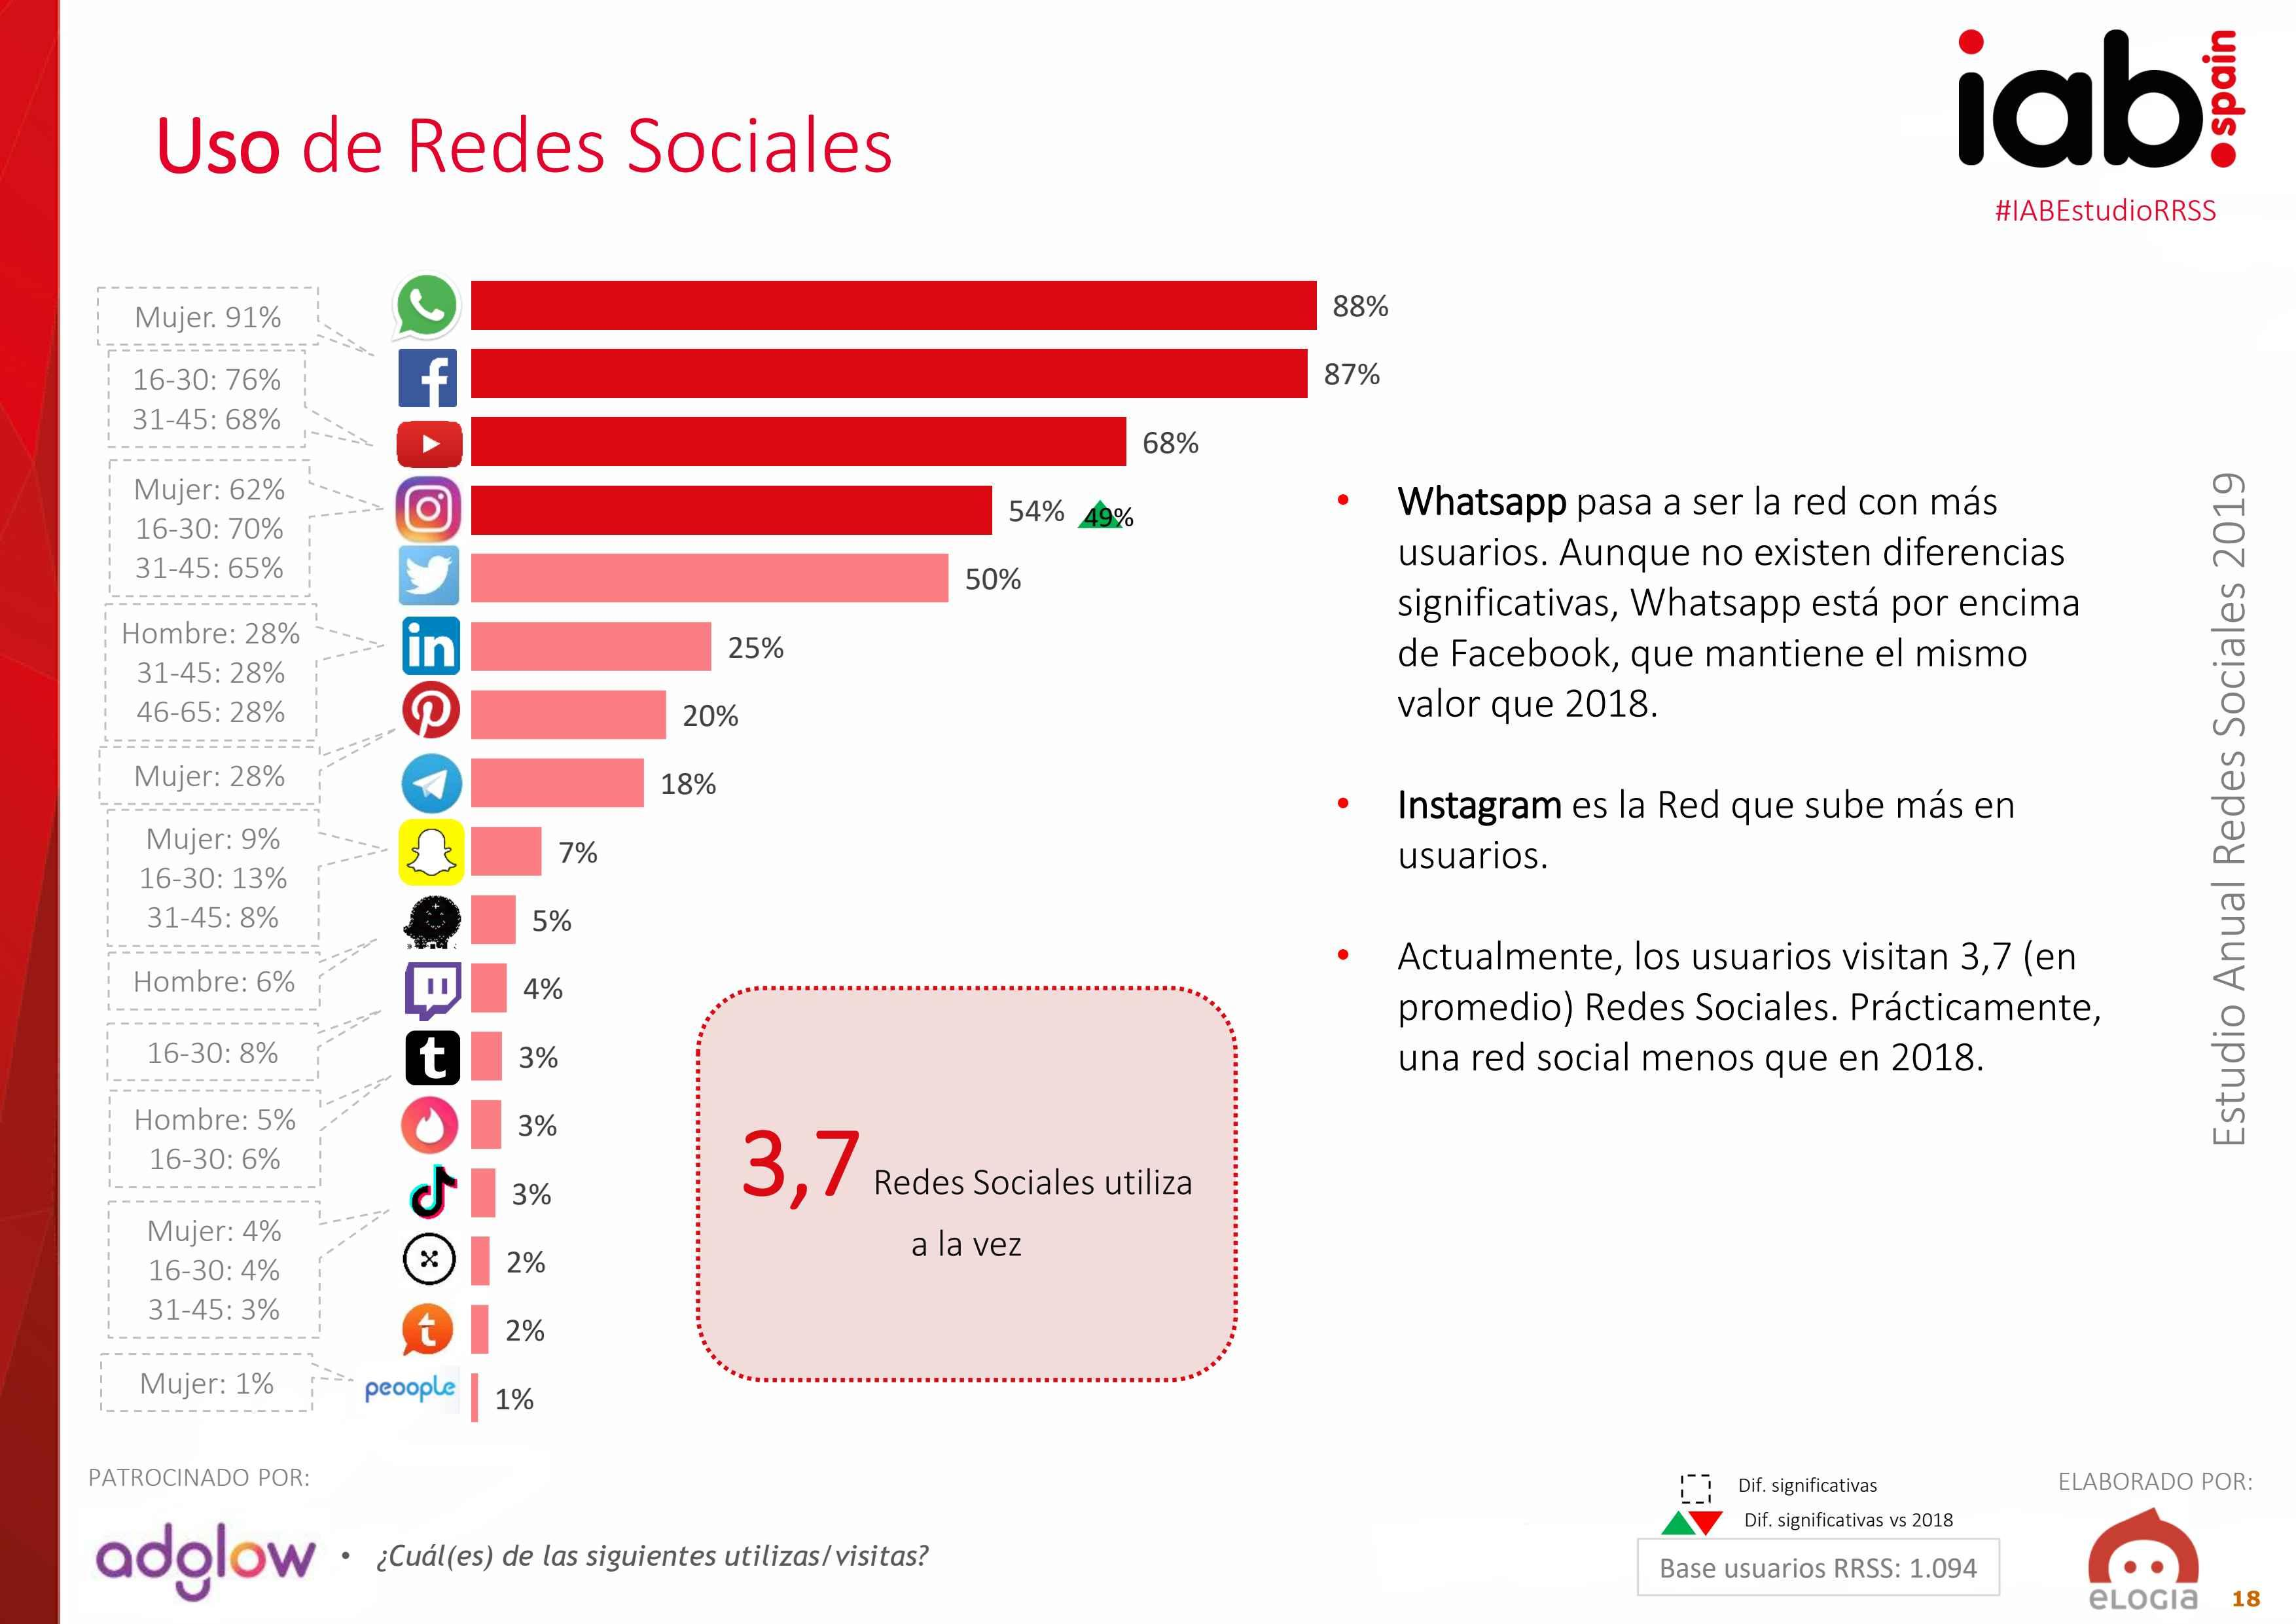
\includegraphics[width=120mm]{uso-redes-iab}}
\end{figure}

En el anterior gráfico horizontal de barras podemos observar el porcentaje de usuarios de redes sociales que utilizan las 17 redes sociales más importantes. Junto a cada barra, podemos encontrar el porcentaje de usuarios correspondiente y, a la izquierda, también encontramos algunos datos en lo que respecta a sexo y algunos grupos de edad. Estos datos proceden de varias encuestas relacionadas con el estudio ``Estudio anual de redes sociales 2019'', realizado el año pasado por IAB Spain.\\

En primer lugar, observamos cómo WhatsApp, la aplicación de mensajería instantánea, encabeza la gráfica, con un volumen de usuarios del 88\%. Muy poco por debajo, con apenas un 1\% menos, le sigue Facebook, la cual es, de hecho, propietaria de WhatsApp. En tercer lugar encontramos YouTube, con un 68\%, que a pesar de ser un porcentaje muy elevado, ya se aleja considerablemente de los dos primeros. Esta cabecera no sorprende, ya que, si miramos datos de años anteriores, Facebook y YouTube han estado la mayor parte del tiempo a la cabeza, y WhatsApp lo ha estado prácticamente desde poco después de su creación.\\

Lo que sí sorprende, es el crecimiento repentino de la red social Instagram, que aumenta un 49\% en usuarios, con respecto al año anterior, posicionándose así por delante de otras como Twitter, LinkedIn, Pinterest o Telegram, con porcentajes que oscilan entre el 18\%y el 50\%. Debajo de estas, encontramos otras redes más pequeñas, como Snapchat, Waze o Twitch, que no tienen un impacto muy significativo en la sociedad digital.

\section{Opinión personal}

Personalmente creo que el usar las redes sociales sea beneficioso o perjudicial para nosotros depende en gran medida del uso que hagamos de ellas. Siempre y cuando hagamos un uso responsable y no abusivo de estas tecnologías, no debería haber ningún problema posterior, y podemos ser usuarios felices. Claro está que esto no elimina por completo las posibilidades de, por ejemplo, ser víctima de ciberacoso, pero si las reduce muy considerablemente. Sé respetuoso con los demás, y los demás serán (o deberían ser) respetuosos contigo.

\section{Conclusiones}

Las redes sociales, como muchas otras cosas, tienen una parte buena y otra mala. Todo depende de cómo las hagamos servir para que tengan un impacto beneficioso o perjudicial en nosotros y en la gente a nuestro alrededor. Por tanto, esta es una serie de consejos que puedes hacer servir para tener una experiencia agradable al hacer uso de las redes sociales:

\begin{itemize}
	\item Haz un uso responsable, y no hagas uso de ellas en situaciones inapropiadas.
	\item No abuses de las redes sociales.
	\item Sé respetuoso con el resto de usuarios, para evitar problemas futuros.
	\item No compartas contenido ni datos personales en las redes, para evitar ser víctima de algún ciberdelito.
	\item Prioriza las relaciones personales antes que las relaciones virtuales. No dejes que las redes te aparten de la sociedad.
\end{itemize}

\end{document}